\documentclass[12pt,a4paper]{article}

\renewcommand*\contentsname{Sadržaj}
\renewcommand{\figurename}{Slika}
\renewcommand{\tablename}{Tabela}
\renewcommand\refname{Reference}
\renewcommand{\arraystretch}{1.25}

\usepackage[margin=0.85in]{geometry}
\usepackage{graphicx}
\usepackage{float}
\usepackage{listings}
\usepackage{multirow}
\usepackage[table]{xcolor}
\usepackage{colortbl}
\usepackage{color}
\usepackage{hyperref}
\usepackage{ctable}
\usepackage{array}
\usepackage{hhline}
\usepackage{caption}
\usepackage{amsfonts}
\usepackage{flowchart}
\usepackage{enumitem}
\usepackage{mathabx}
\usepackage{amssymb}
\usepackage{titlesec}
\usetikzlibrary{arrows}

\lstloadlanguages{C,C++,csh,Java}

\definecolor{red}{rgb}{0.6,0,0} 
\definecolor{blue}{rgb}{0,0,0.6}
\definecolor{green}{rgb}{0,0.8,0}
\definecolor{cyan}{rgb}{0.0,0.6,0.6}
\definecolor{magnolia}{rgb}{0.97, 0.96, 1.0}
\definecolor{colora}{rgb}{0.67, 0.8, 0.94}
\definecolor{colorb}{rgb}{0.67, 0.94, 0.82}
\definecolor{colord}{rgb}{0.67, 0.9, 0.93}
\definecolor{colore}{rgb}{0.6, 0.73, 0.89}
\definecolor{colorf}{rgb}{0.61, 0.87, 1.0}
\definecolor{grey}{rgb}{0.75, 0.75, 0.75}
\definecolor{amber}{rgb}{1.0, 0.75, 0.0}

\lstset{
language=csh,
basicstyle=\footnotesize\ttfamily,
numbers=left,
numberstyle=\tiny,
numbersep=5pt,
tabsize=2,
extendedchars=true,
breaklines=true,
frame=b,
stringstyle=\color{blue}\ttfamily,
showspaces=false,
showtabs=false,
xleftmargin=17pt,
framexleftmargin=17pt,
framexrightmargin=5pt,
framexbottommargin=4pt,
commentstyle=\color{green},
morecomment=[l]{//}, %use comment-line-style!
morecomment=[s]{/*}{*/}, %for multiline comments
showstringspaces=false,
morekeywords={ abstract, event, new, struct,
as, explicit, null, switch,
base, extern, object, this,
bool, false, operator, throw,
break, finally, out, true,
byte, fixed, override, try,
case, float, params, typeof,
catch, for, private, uint,
char, foreach, protected, ulong,
checked, goto, public, unchecked,
class, if, readonly, unsafe,
const, implicit, ref, ushort,
continue, in, return, using,
decimal, int, sbyte, virtual,
default, interface, sealed, volatile,
delegate, internal, short, void,
do, is, sizeof, while,
double, lock, stackalloc,
else, long, static,
enum, namespace, string},
keywordstyle=\color{cyan},
identifierstyle=\color{red},
backgroundcolor=\color{magnolia},
}

\DeclareCaptionFont{white}{\color{white}}
\DeclareCaptionFormat{listing}{\colorbox{blue}{\parbox{\textwidth}{\hspace{15pt}#1#2#3}}}
\captionsetup[lstlisting]{format=listing,labelfont=white,textfont=white, singlelinecheck=false, margin=0pt, font={bf,footnotesize}}

\newcolumntype{a}{>{\columncolor{colora}}c}
\newcolumntype{b}{>{\columncolor{colorb}}c}
\newcolumntype{d}{>{\columncolor{colord}}c}
\newcolumntype{e}{>{\columncolor{colore}}c}
\newcolumntype{f}{>{\columncolor{colorf}}c}
\newcolumntype{P}[1]{>{\centering\arraybackslash}p{#1}}
\newcolumntype{?}{!{\vrule width 1pt}}

\begin{document}

\begin{titlepage}
	\centering
	{\scshape Univerzitet u Sarajevu \par}
	{\scshape Elektrotehnički Fakultet \par}
	{\scshape Odsjek za Računarstvo i Informatiku \par}
	\vspace{2cm}
	{\Large\scshape Praktikum: Poslovni Informacioni Sistemi\par}
	\vspace{2.5cm}
	{\huge\bfseries \textit{Service Requirements Specification} Dokument\par}
	\vspace{2.5cm}
	\Large Studenti: \par
	{\Large\itshape \textsc{Bojadžić} Hanna, 1421/17311\par}
	{\Large\itshape \textsc{Građanin} Ehvan, 1438/17335\par}
	{\Large\itshape \textsc{Halilbegović} Kemal, 1469/16682\par}
	{\Large\itshape \textsc{Krupalija} Ehlimana, 1431/17461\par}
	{\Large\itshape \textsc{Kubat} Ismar, 1422/17148\par}
	{\Large\itshape \textsc{Kulović} Nejra, 1519/17484\par}
	{\Large\itshape \textsc{Muftić} Belma, 1423/17260\par}
	{\Large\itshape \textsc{Pribišić} Tarik, 1536/2018\par}
	\vfill
	Predmetni nastavnik:\par
	doc. dr. \textsc{Anel Tanović}, dipl. ing. el.
	\vfill
	{\large Juni, 2019\par}
\end{titlepage}

\pagenumbering{gobble}

\tableofcontents

\newpage

\pagenumbering{arabic}

\section{ITIL procesi}

\subsection{\textit{Change Management}}

\quad Upravljanje promjenama je ITIL (\textit{Information Technology Infrastructure Library}) proces koji pripada skupu procesa u okviru tranzicije usluga. Njegova svrha je upravljanje promjenama koje se dešavaju nad nekim IT servisom, te olakšavanje prilagođavanja promjenama, kao i njihovom uvođenju i što boljem procesiranju zahtjeva za promjenama. U prvim verzijama ITIL-a promjene su bile generičke, no u kasnijim verzijama (od verzije 3 nadalje) prepoznata je potreba za uvođenjem tzv. modela promjena, koji razdvajaju promjene u različite kategorije prema značaju i hitnosti.

Pri upravljanju promjenama potrebno je definisati sljedeće pojmove:

\begin{enumerate}
\item \textbf{Zahtjev za promjenom (\textit{Request for Change - RFC})} - trebaju postojati jasno definisani slučajevi u kojima se prepoznaje potreba za vršenjem promjena. Promjene mogu inicirati osobe od interesa (\textit{stakeholderi}, ukoliko je u pitanju IT usluga koju koristi neka kompanija i sl.), ili mogu biti vođene odzivom sistema, odnosno inicirane zbog grešaka, pogrešnog ili slabog korištenja nekih dijelova sistema. Zbog toga je važno omogućiti različitim osobama od interesa iniciranje promjena, kao i osigurati da se vrši praćenje korištenja sistema te analiza uspješnosti i frekvencije korištenja istog.

\item \textbf{Promjena} -  moguće je vršiti različite akcije nad sistemom koje se smatraju promjenom: dodavanje novih komponenti, izmjenu ili potpuno uklanjanje starih, spajanje različitih funkcionalnosti i mnoge druge. Različite vrste promjena trebaju se tretirati na različite načine. Potrebno je jasno definisati šta je moguća promjena, koja je njena kategorija, koliki je njen prioritet te ko je zadužen za implementaciju iste.

\item \textbf{Osoblje za upravljanje promjenama} - treba postojati jasno definisana uloga za osobe koje će moći nadzirati promjene, odobravati vršenje istih ili odbacivati prijedloge. Od ovog osoblja očekuje se da je u stanju brzo i adekvatno reagovati na hitne promjene, kao i da izvrši ispravno rasuđivanje da li će neka promjena pozitivno ili negativno utjecati na sam sistem (potrebno je izvršiti analizu koja se dokumentuje u vidu \textit{Projected Service Outage - PSO} dokumenta, u kojem su izlistane sve predvidljive devijacije od plana promjena).
\end{enumerate}

Upravljanje promjenama sastoji se od četiri osnovna podprocesa:

\begin{enumerate}
\item \textbf{Filtriranje promjena}, u okviru kojeg se pregledaju svi primljeni zahtjevi za vršenje promjena, analiziraju se i vrši se odluka koji zahtjevi će se prihvatiti, a koji zahtjevi će se odbiti, uz što se prilaže PSO dokument.

\item \textbf{Savjetovanje sa CAB (\textit{Change Advisory Board} i komitetom za hitne promjene}, što se odnosi na argumentovanje prethodno utvrđenih zahtjeva koji su prepoznati kao neophodni, te predstavljanje tih argumenata savjetima i komitetima koji jedini imaju autoritet za odobravanje promjena. Tek nakon što se promjene odobre, počinje se sa njihovom implementacijom. U svakom drugom slučaju, promjene se odbacuju.

\item \textbf{Upravljanje promjenama}, što se odnosi na dodjeljivanje posla zaposlenicima ovisno o vrsti zahtjeva koji je potrebno ispuniti te praćenje rada na dodavanju novih, zamjenom ili uklanjanjem postojećih funkcionalnosti u skladu s postojećim zahtjevima. Upravljanje promjenama vrši se stalno, od početka do kraja procesa njihovog uvođenja u sistem.

\item \textbf{Izvještavanje o promjenama}, odnosno kreiranje izvještaja o svakoj izvršenoj promjeni, što uključuje argumente za i protiv vršenja promjena, PSO dokument, dozvolu od CAB i drugih komiteta, kao i izvještaj o samom procesu implementacije i uvođenja promjena te kako je uvođenje istih u sistem promijenilo poslovanje, tj. da li je uvođenje promjena imalo pozitivan efekat ili ne.

\end{enumerate}

\subsection{\textit{Event Management}}

\quad Upravljanje događajima je ITIL (\textit{Information Technology Infrastructure Library}) proces koji pripada skupu procesa u okviru upravljanja uslugama. Njegova svrha je da nadzire sve značajne događaje u sistemu, detektuje nove i procesira ih na adekvatan način. Ovaj proces u \textit{ITIL}-u 2011 povezan je sa upravljanjem pristupom preko interfejsa, budući da su ta dva procesa u bliskoj korelaciji: u sistemu koji nadzire važne, često sigurnosno osjetljive događaje, onemogućavanje neautorizovanog pristupa jedan je od najvažnijih zahtjeva. \\

Pri upravljanju događajima potrebno je definisati sljedeće pojmove:

\begin{enumerate}
\item \textbf{Događaj} - u kompleksnim sistemima postoje različite vrste događaja i notifikacija, te je potrebno napraviti razgraničenje kojim vrstama događaja se bavi sistem upravljanjem događajima (događaji se najčešće dijele na informacije, upozorenja i greške).

\item \textbf{Prioritet} - različiti događaji imaju različit značaj, pri čemu je neke događaje potrebno hitno procesirati, dok drugi događaji mogu čekati određeno vrijeme. Iz tog razloga neophodno je svim vrstama događaja dodijeliti određene prioritete, koji se najčešće označavaju brojevima.

\item \textbf{Odziv} - sistem najčešće treba reagovati na događaje, posebno ukoliko je njihov prioritet veliki. Iz tog razloga potrebno je definisati vrstu i vrijeme odziva na različite događaje, te način njihovog procesiranja.
\end{enumerate}

Upravljanje događajima sastoji se od četiri osnovna podprocesa:

\begin{enumerate}
\item \textbf{Korištenje mehanizama za nadzor događaja}, koji se odnosi na stalnu mogućnost sistema da detektuje događaje, kao i da nadzire postojeće događaje i vrši njihovo procesiranje. Budući da je broj događaja koji konstantno ulaze u sistem veoma veliki, vrlo je važno ispravno izvršiti diferenciranje na različite vrste događaja, kako se ne bi detektovao veliki broj nevažnih ili nekritičnih događaja. S druge strane, sistem mora biti u mogućnosti reagovati na događaje na adekvatan način, posebno u slučaju kad se više različitih događaja treba procesirati u isto vrijeme.

\item \textbf{Prvi nivo korelacije: \textit{Filtriranje događaja}}, odnosno analiza događaja kako bi se odredilo da li je događaj relevantan za sistem ili ne. Ukoliko je događaj samo informacija, najčešće nije potrebno vršiti nikakve akcije te se takvi događaji mogu ignorisati. No, upozorenja i greške se moraju procesirati na adekvatan način, te je vrlo važno imati adekvatne mehanizme kako takvi događaji ne bi bili ignorisani (ali i kako informacije ne bi bile procesirane, ukoliko to nije neophodno).

\item \textbf{Drugi nivo korelacije: \textit{Izbor odziva}}, odnosno dalja analiza događaja koji nisu filtrirani na prethodnom nivou. Budući da je za upozorenja i greške najčešće potrebno imati adekvatan odziv, na ovom nivou potrebno je odrediti da li odziv može biti automatski (u pitanju je neki od poznatih događaja za koje postoje predefinisani koraci odziva), ili je potrebno eskalirati situaciju na viši nivo.

\item \textbf{Pregled događaja i njegovo zatvaranje}, koji se odnosi na dodatnu provjeru aktivnih događaja koji se trenutno nadziru. Ukoliko je automatska akcija bila dovoljna da se događaj procesira na adekvatan način i stanje vrati u normalno, te ukoliko je sistem proslijedio informacije o događaju individuama sistema koji su ga procesirali na adekvatan način, takav događaj moguće je zatvoriti, kako bi se novi događaji mogli procesirati bez čekanja.
\end{enumerate}

\newpage

\section{Opis i namjena sistema}

\subsection{Osnovne informacije o kompaniji}

\quad Kompanija \textbf{Idea d.o.o. Sarajevo} je mlada kompanija koja se bavi razvojem i održavanjem informacionih sistema za državne institucije, poput Zavoda za izgradnju Kantona Sarajevo, Zavoda za informatiku i statistiku Kantona Sarajevo, Direkcije za robne rezerve Kantona Sarajevo i mnogih drugih. Ovi informacioni sistemi omogućavaju pregled svih zaposlenika, njihovih personalnih dosijea (uključujući lične podatke, razne vrste dokumenata, rješenja i ugovora) te iniciranje različitih akcija, poput slanja na seminare, edukacije i stručna usavršavanja, vršenje ocjenjivanja radnika, donošenje različitih vrsta rješenja te vršenje sistematizacije. \\

Softver koji je razvijen potrebno je svakodnevno održavati. Korisnici sistema su najčešće srednje životne dobi, bez tehničkog znanja na visokom nivou, te se svakodnevno susreću s različitim poteškoćama u korištenju sistema. Ponekad dolazi do pojave grešaka, na koje je potrebno što prije reagovati, kako se ne bi ugrozilo ispravno i kontinualno funkcionisanje sistema. Same institucije često šalju zahtjeve za promjenama sistema, zbog stalnog donošenja novih odredbi te izmjene starih, zbog čega je sistem potrebno stalno ažurirati kako bi odgovarao trenutnom stanju i olakšavao poslovanje ovih instituacija. \\

Iz svih ovih razloga, Idea d.o.o. Sarajevo ima potrebu za razvojem aplikacije koja će im omogućiti upravljanje događajima i promjenama u sistemu. Ovakva aplikacija olakšati će detekciju grešaka i zahtjeva za promjenama, ubrzati reagovanje na hitne promjene te osigurati da sistem kontinualno funkcioniše bez problema, te da njegovi korisnici mogu imati pouzdano i ažurirano okruženje u kojem će im biti jednostavno raditi.

\subsection{Poslovni procesi}

\quad Kompanija želi informacioni sistem koji omogućava sljedeće funkcionalnosti:

\begin{itemize}
\renewcommand\labelitemi{$\square$}
\item Pregled svih zahtjeva za promjenama od strane tima za upravljanje promjenama;
\item Pisanje izvještaja (PSO dokumenta) o predloženoj promjeni te slanje istog komitetu za promjene na pregled;
\item Konačno odobravanje ili odbijanje promjena od strane komiteta za promjene;
\item Prihvatanje i odbijanje promjena, te njihovo označavanje kompletiranim nakon implementacije;
\item Slanje promjena timu za produkciju;
\item Prijavljivanje grešaka i problema pri implementaciji od strane tima za produkciju;
\item Pregled statističke analize korištenja sistema, uz informacije o slabo ili nikako korištenim dijelovima;
\item Prijava problema pri korištenju od strane korisnika sistema koji firma održava.
\end{itemize}

Sve ove funkcionalnosti trebaju biti objedinjene u jednoj aplikaciji, te mora biti osigurana sigurnost i konzistentnost podataka. U nastavku će biti prikazane osnovne informacije vezane za ITIL procese pomoću kojih je moguće modelirati poslovne procese sistema za koji je potrebno napraviti aplikaciju.

\subsubsection{Upravljanje promjenama}

\quad Sama svrha sistema je praćenje korištenja softvera koji se održava te prijem i procesiranje zahtjeva za promjene. U skladu s tim, definišu se dvije kategorije promjena:

\begin{itemize}
\renewcommand\labelitemi{-}
\item \textit{Obične promjene}, odnosno promjene koje inicijalizira tim za upravljanje promjenama na osnovu zahtjeva koje šalju državne institucije formalnim putem (van samog sistema za upravljanje promjenama), ili koje tim za upravljanje promjenama ocijeni neophodnim na osnovu statističke analize korištenja sistema (slabo ili nikako korišteni dijelovi sistema);
\item \textit{Hitne promjene}, koje se detektuju na osnovu prijave problema pri korištenju od strane korisnika sistema koje firma održava. Prijava problema korisnicima je omogućena unutar same aplikacije.
\end{itemize}

Osim kategorija, promjene imaju i svoje vrste, kako slijedi:

\begin{itemize}
\renewcommand\labelitemi{-}
\item Dodavanje novih komponenti;
\item Izmjena postojećih komponenti;
\item Brisanje postojećih komponenti.
\end{itemize}

Svaka promjena mora imati definisanu kategoriju i vrstu. Osoblje za upravljanje promjenama vrši njihov pregled i filtriranje - zahtjev se analizira, te se ili odbija uz obrazloženje, ili se šalje komitetu za promjene na dodatnu analizu i odobravanje. Komitet za promjene ima mogućnost pregleda svih promjena koje su im poslane od strane tima za upravljanje promjenama, te odbijanje ili odobravanje promjena. Te informacije prosljeđuju se timu za upravljanje promjenama, te ukoliko se odobri vršenje promjena, iste se dodjeljuju jednom od dostupnih timova za razvoj softvera. \\

Na osnovu ovih informacija, moguće je dodijeliti određene funkcionalnosti sistema različitim vrstama korisnika, na način kako slijedi:

\begin{itemize}
\renewcommand\labelitemi{$\square$}
\item Pregled svih zahtjeva za promjenama - \textcolor{blue}{tim za upravljanje promjenama};
\item Pisanje izvještaja (PSO dokumenta) o predloženoj promjeni te slanje istog komitetu za promjene na pregled - \textcolor{blue}{tim za upravljanje promjenama};
\item Prihvatanje i odbijanje promjena, te njihovo označavanje kompletiranim nakon implementacije - \textcolor{blue}{tim za upravljanje promjenama};
\item Konačno odobravanje ili odbijanje promjena - \textcolor{green}{komitet za promjene};
\item Slanje promjena timu za produkciju - \textcolor{blue}{tim za upravljanje promjenama};
\item Pregled statističke analize korištenja sistema, uz informacije o slabo ili nikako korištenim dijelovima - \textcolor{blue}{tim za upravljanje promjenama}.
\end{itemize}

\subsubsection{Upravljanje događajima}

\quad Događaje u sistemu predstavljaju prijave problema od strane korisnika sistema koji se održavaju, ili od strane razvojnog tima koji vrši implementaciju izmjena u sistemu. Pregled i nadziranje događaja vrši tim za upravljanje promjenama, dok korisnici sistema i razvojni tim mogu vršiti iniciranje novih događaja. \\

U skladu s ovim, potrebno je izvršiti definisanje svih različitih događaja u sistemu, njihovih tipova i prioriteta, što je prikazano u Tabeli \ref{tabela1}.

\begin{table}[H]
\centering
\begin{tabular}{| c | c | c |} \hline
\cellcolor{gray!25}\textbf{Vrsta događaja}		& \cellcolor{gray!25}\textbf{Inicijator}			& \cellcolor{gray!25}\textbf{Prioritet} 		\\ \hline
Greška u sistemu										& \cellcolor{green!25}Korisnik						& \cellcolor{blue!15}3							\\ \hline
Pogrešno korištenje sistema							& \cellcolor{green!25}Korisnik						& \cellcolor{blue!15}1							\\ \hline
Nemogućnost implementacije promjene			& \cellcolor{green!25}Razvojni tim					& \cellcolor{blue!15}2							\\ \hline
Greška nakon uvođenja promjena					& \cellcolor{yellow!25}Korisnik						& \cellcolor{blue!35}3							\\ \hline
Greška pri testiranju sistema							& \cellcolor{red!25}Razvojni tim					& \cellcolor{blue!55}2							\\ \hline
\end{tabular}
\caption{Svi događaji sistema}
\label{tabela1}
\end{table}

Svi događaji prikazuju se timu za upravljanje promjenama, koji vrše odziv na događaje, na jedan od tri načina:

\begin{itemize}
\renewcommand\labelitemi{-}
\item \textit{Otkazivanje promjena}, koje se vrši ukoliko razvojni tim prijavi da nije u mogućnosti da implementira promjene iz nekog razloga (poput samog načina na koji sistem funkcioniše, nedovoljnog broja informacija o samoj promjeni koju je potrebno izvršiti, nemogućnosti povezivanja sa postojećim sistemom i sl.).
\item \textit{Slanje razvojnom timu na popravljanje}, koje se vrši ukoliko korisnici prijave grešku u sistemu prije ili nakon uvođenja promjena ili ukoliko dođe do greške pri testiranju sistema.
\item \textit{Organizacija edukacije korisnika ili razgovor s korisnikom}, koji se vrše ukoliko korisnik prijavi da ne zna kako ispravno koristiti sistem.
\end{itemize}

Na osnovu ovih informacija, moguće je dodijeliti određene funkcionalnosti sistema različitim vrstama korisnika, na način kako slijedi:

\begin{itemize}
\renewcommand\labelitemi{$\square$}
\item Prijavljivanje grešaka i problema pri implementaciji promjena - \textcolor{red}{razvojni tim};
\item Prijava problema pri korištenju sistema koji firma održava - \textcolor{brown}{korisnici sistema koji se održava}.
\end{itemize}

\newpage

\subsection{Pregled slučajeva upotrebe}

\quad Slučajevi upotrebe sistema koji odgovaraju funkcionalnostima vezanim za upravljanje promjenama prikazani su na Slici \ref{useCase1}. Akteri sistema su tim za upravljanje promjenama, komitet za promjene i tim za produkciju, koji učestvuju u realizaciji slučajeva upotrebe.

\begin{figure}[H]
\center
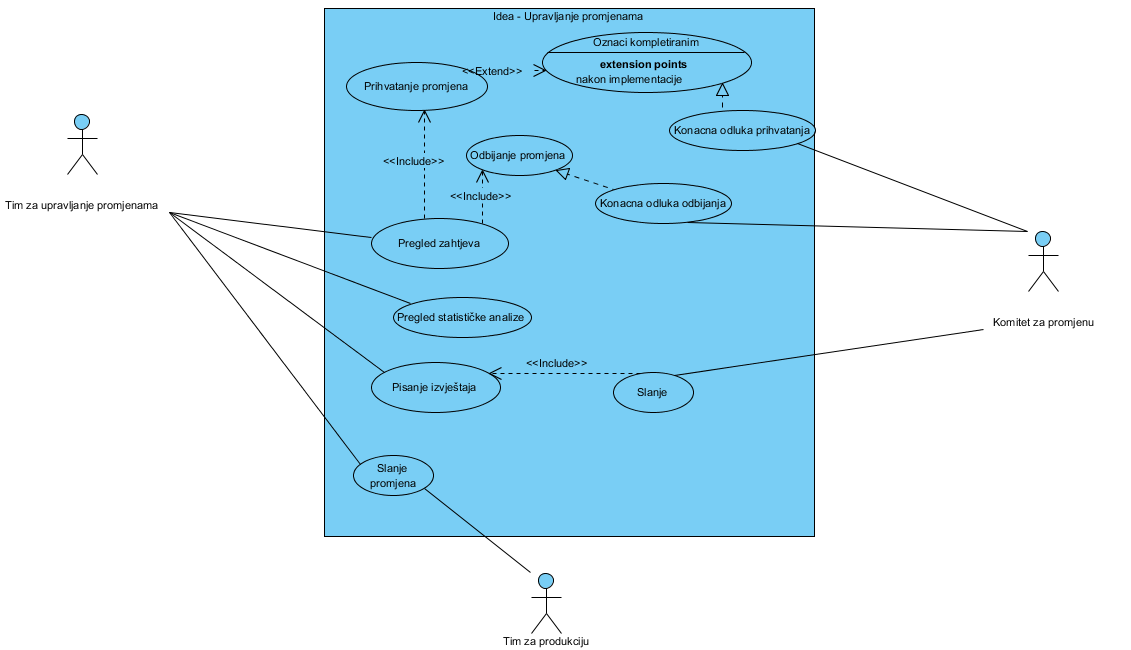
\includegraphics[scale=0.4]{../res/useCase1.PNG}
\caption{Dijagram slučajeva upotrebe za upravljanje promjenama u sistemu}
\label{useCase1}
\end{figure}

Slučajevi upotrebe sistema koji odgovaraju funkcionalnostima vezanim za upravljanje događajima prikazani su na Slici \ref{useCase2}. Akteri sistema su korisnici sistema i tim za produkciju, koji učestvuju u realizaciji slučajeva upotrebe.

\begin{figure}[H]
\center
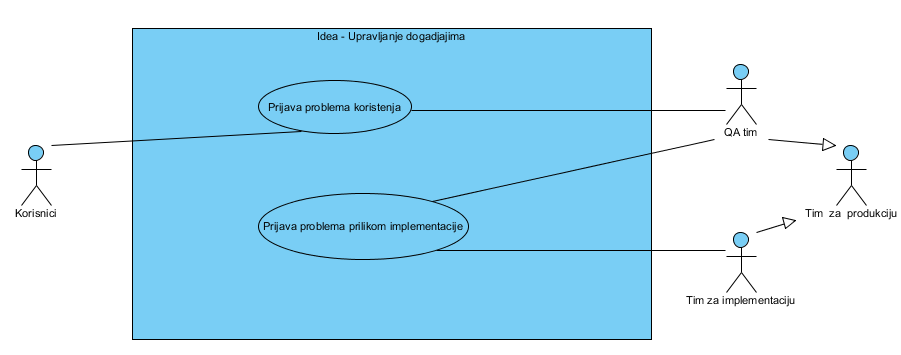
\includegraphics[scale=0.45]{../res/useCase2.PNG}
\caption{Dijagram slučajeva upotrebe za upravljanje događajima u sistemu}
\label{useCase2}
\end{figure}

\newpage

\subsection{Metodologija razvoja sistema}

\quad Za razvoj sistema biti će korištena SCRUM metodologija, koja predstavlja jednu od najpoznatijih agilnih metodologija za razvoj softvera. Razvoj sistema obavljati će se u sprintovima, sa trajanjem svakog sprinta od po 7 dana, pri čemu će se funkcionalnosti sistema razdvojiti prema korisničkim ulogama. Dodatno, \textit{task}-ovi će biti razdvojeni na \textbf{\textit{frontend}} i \textbf{\textit{backend}} \textit{task}ove, a novi zadaci biti će dodavani po potrebi (ovisno o mogućnostima raspodjele većih zadataka na manje podzadatke). \\

Inicijalni \textit{Trello Board} prikazan je na Slici \ref{trello1} i \ref{trello2}. Na slikama je vidljivo da su zadaci podijeljeni u nekoliko različitih grupa:

\begin{itemize}
\renewcommand\labelitemi{-}
\item \textit{To-do} - skup svih zadataka koje je potrebno izvršiti;
\item \textit{In progress} - skup zadataka koji su ocijenjeni najvažnijim po određenom kriteriju (vrijeme isporuke ili kritičnost za sistem), te koji se trenutno izvršavaju;
\item \textit{Testing} - skup zadataka koji su implementirani no potrebno je izvršiti njihovu verifikaciju;
\item \textit{Resolving bugs} - skup zadataka iz prethodnih inkremenata u kojima su pronađene greške, te koje se trenutno ispravljaju;
\item \textit{Done} - skup svih zadataka koji su uspješno završeni.
\end{itemize}

Zadaci se dijele u tri skupine:
\begin{enumerate}
\item \textcolor{blue}{\textit{Documentation}}, što se odnosi na pisanje dokumentacije vezane za projekat;
\item \textcolor{amber}{\textit{Backend}}, što se odnosi na implementaciju funkcionalnosti te perzistencije podataka;
\item \textcolor{orange}{\textit{Frontend}}, što se odnosi na implementaciju korisničkog interfejsa.
\end{enumerate}

\begin{figure}[H]
\center
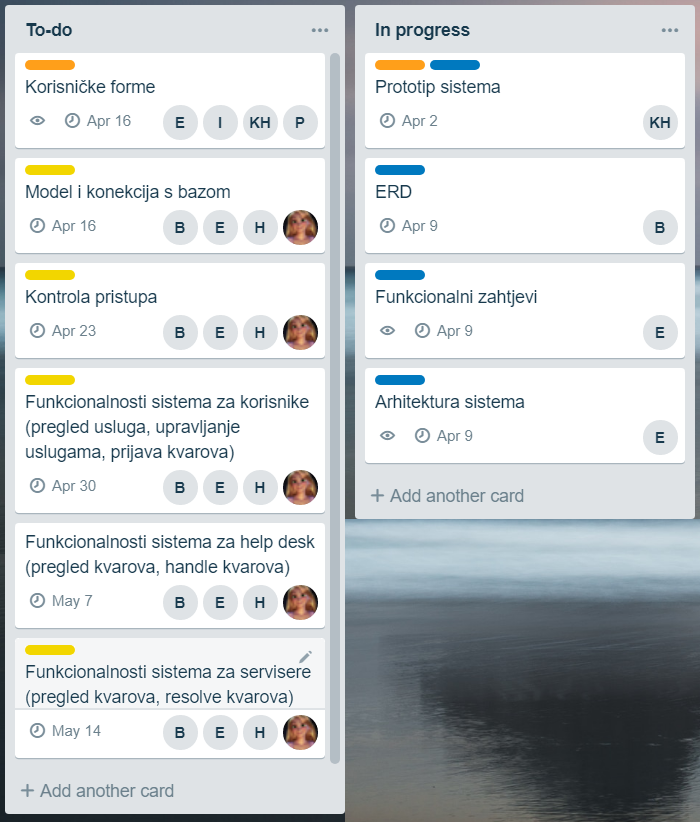
\includegraphics[scale=0.6]{../res/trello1.PNG}
\caption{\textit{Trello board} projekta, zadaci koji se trebaju izvršiti i koji se trenutno izvršavaju}
\label{trello1}
\end{figure}

\begin{figure}[H]
\center
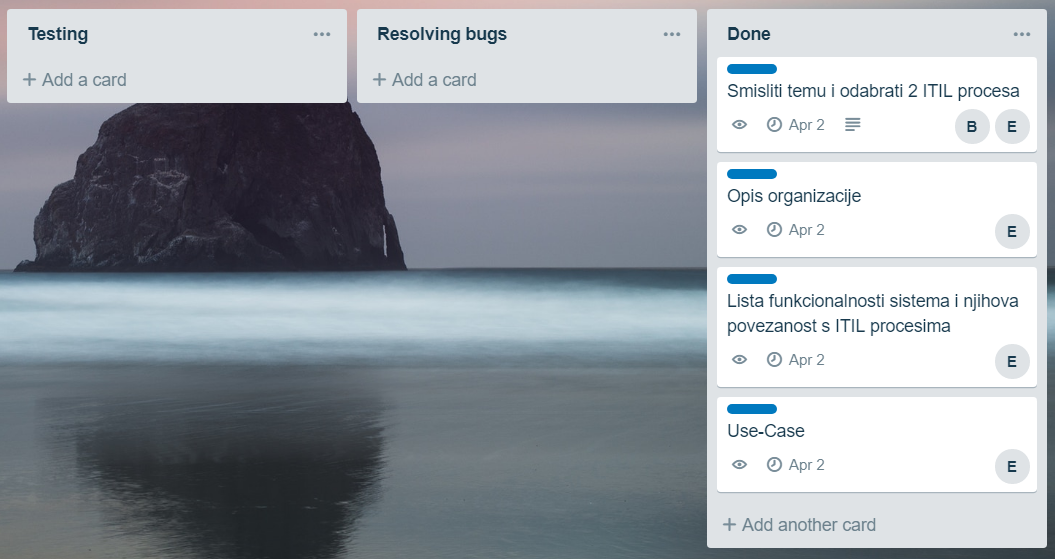
\includegraphics[scale=0.6]{../res/trello2.PNG}
\caption{\textit{Trello board} projekta, zadaci koji su završeni te dijelovi sistema koji se testiraju ili popravljaju}
\label{trello2}
\end{figure}

\newpage

\subsection{Prototip sistema}

\quad Na Slici \ref{pt1} prikazan je osnovni izgled ekrana aplikacije, koja ima korisnički interfejs kreiran poštujući pravila dobrog  dizajna.

\begin{figure}[H]
\center
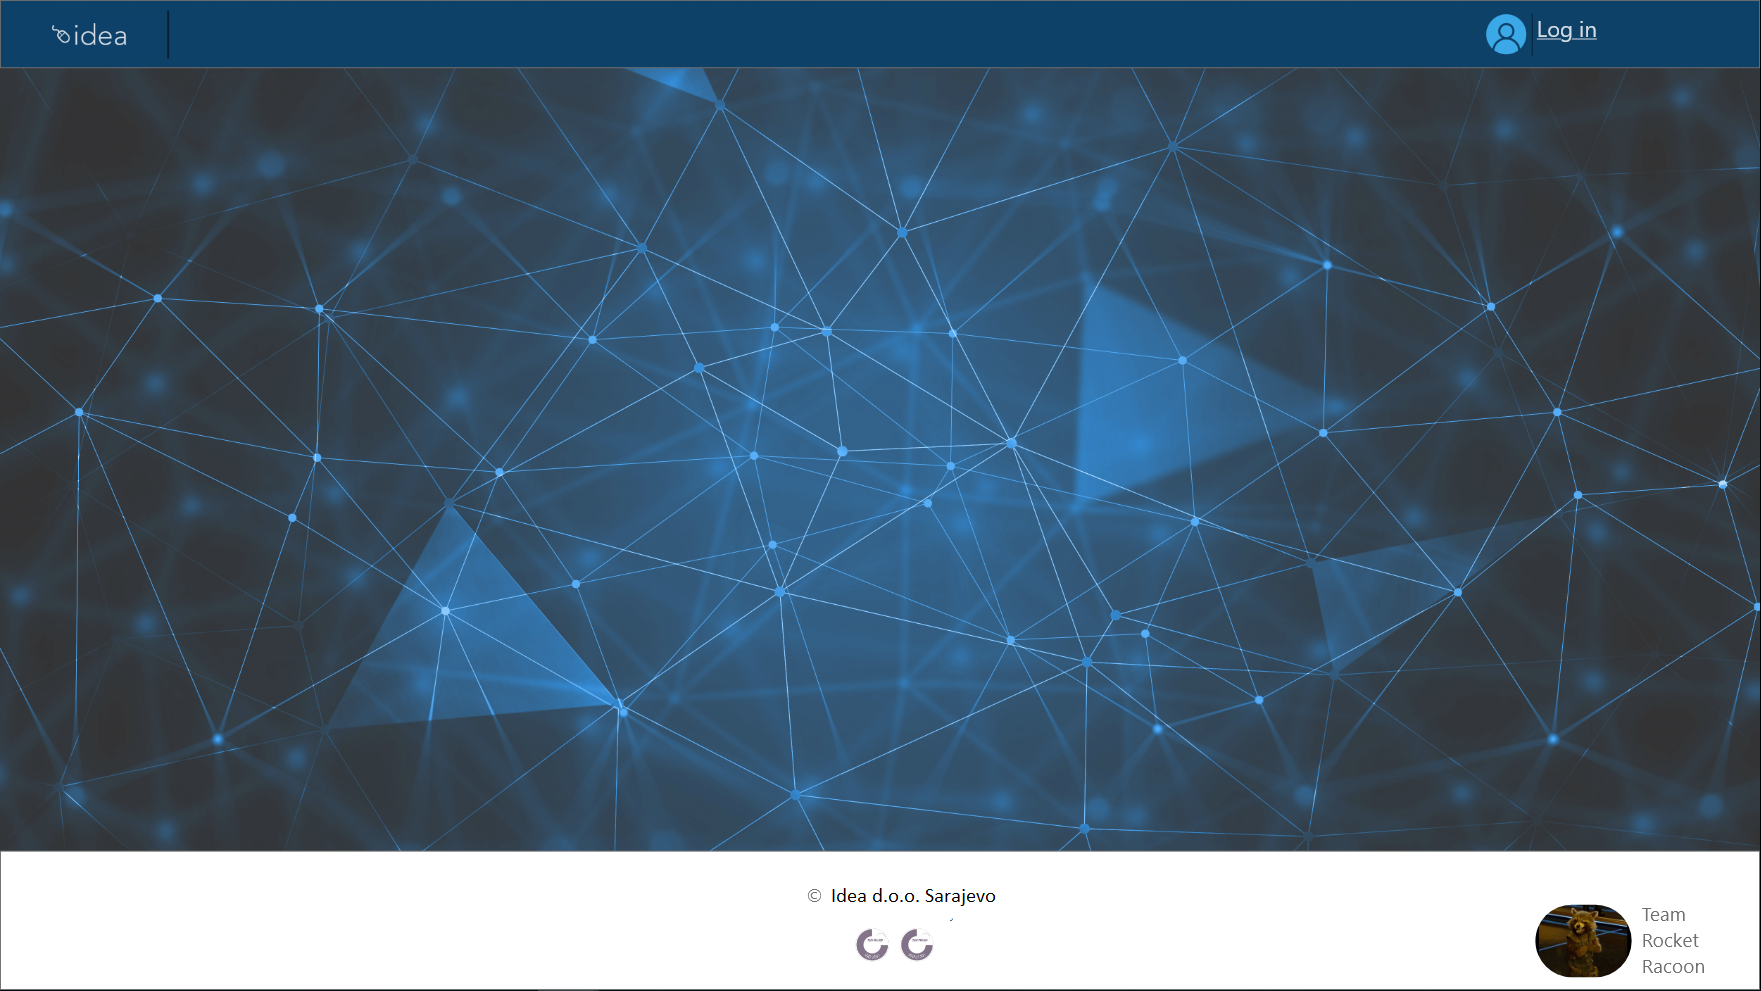
\includegraphics[scale=0.4]{../res/Prototype/Main.PNG}
\caption{Osnovni izgled ekrana aplikacije}
\label{pt1}
\end{figure}

Na Slici \ref{pt2} prikazan je izgled interfejsa za unos korisničkih podataka, nakon čega se omogućava pristup aplikaciji za različite vrste korisnika.

\begin{figure}[H]
\center
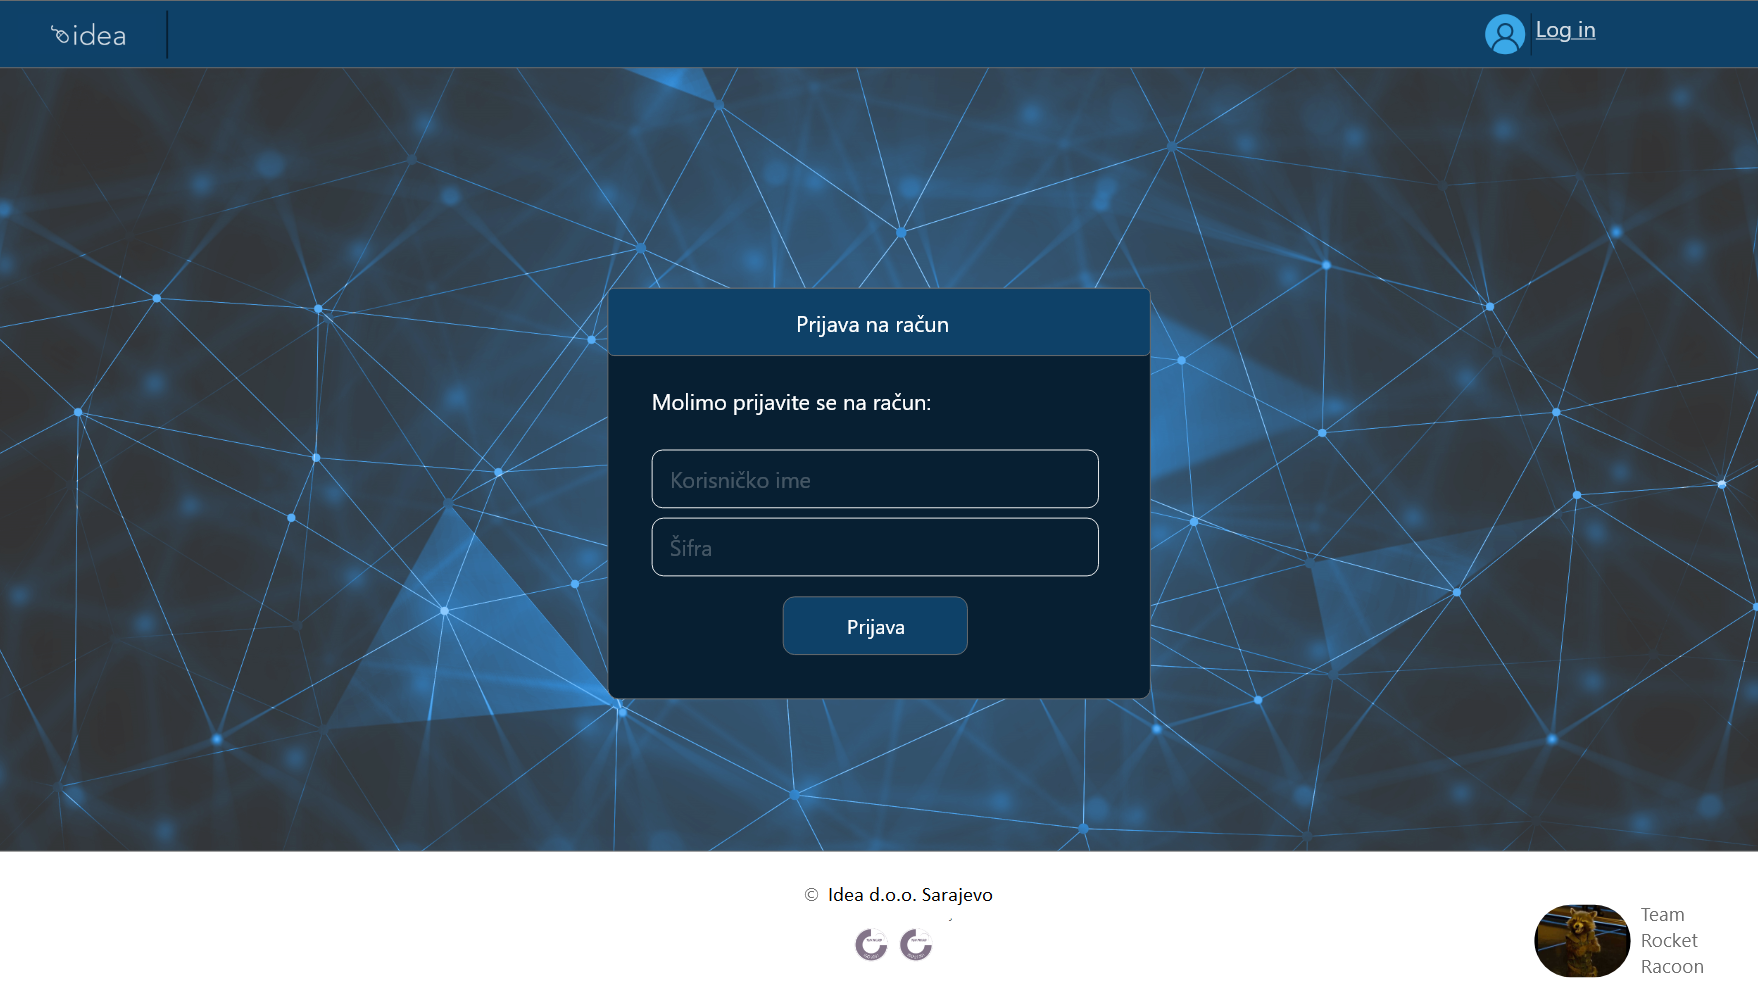
\includegraphics[scale=0.4]{../res/Prototype/LogIn.PNG}
\caption{Izgled interfejsa za unos korisničkih podataka}
\label{pt2}
\end{figure}

\newpage

Na Slici \ref{pt3} prikazan je izgled ekrana za pregled svih zahtjeva za promjenama, koje može vršiti tim za upravljanje promjenama. Nakon pregleda promjene, vrši se njena analiza i \textit{upload}-uje se PSO dokument, te se pritiskom na dugme \textbf{Prihvati} promjena automatski šalje komitetu za promjene. Alternativno, promjena se može odmah odbiti.

\begin{figure}[H]
\center
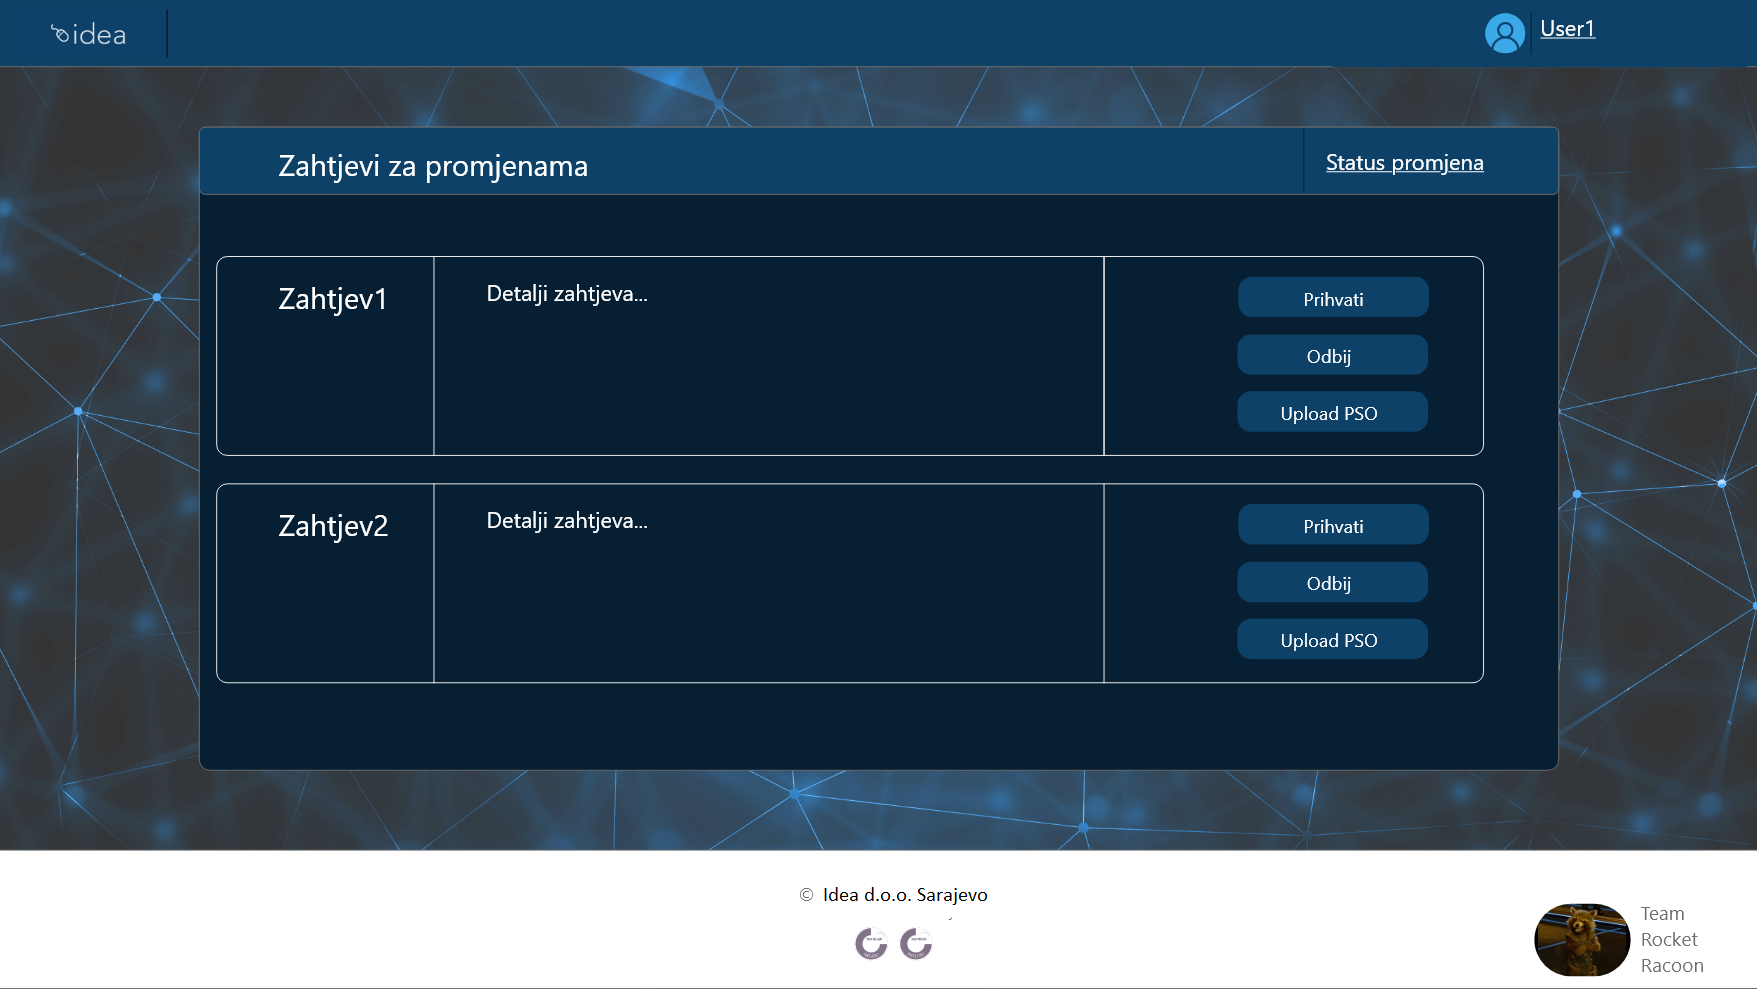
\includegraphics[scale=0.4]{../res/Prototype/Zahtjev-promjene.PNG}
\caption{Izgled interfejsa za pregled i procesiranje promjena}
\label{pt3}
\end{figure}

Na Slici \ref{pt4} prikazan je izgled ekrana za pregled svih odobrenih promjena, koje može vršiti tim za upravljanje promjenama. Promjene se mogu poslati razvojnom timu, te se vršiti njihov kontinualni nadzor i otkazivanje, ukoliko se pokaže da je promjenu nemoguće, vrlo teško ili neisplativo ugraditi u sistem.

\begin{figure}[H]
\center
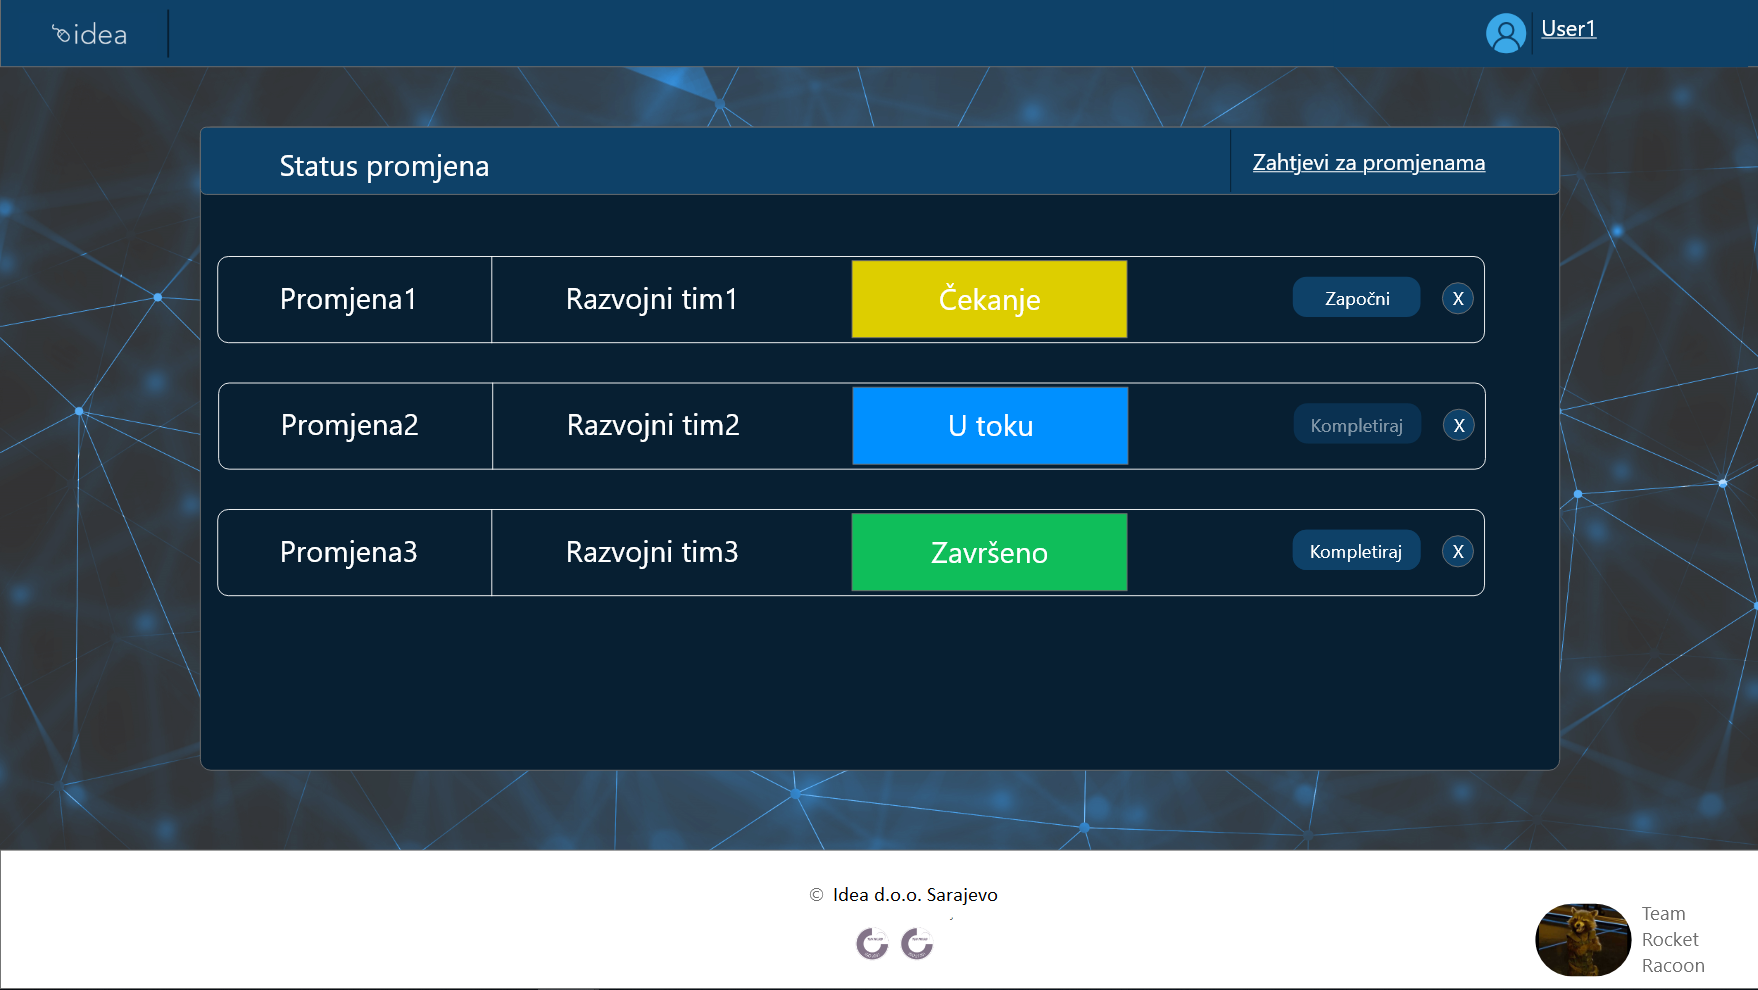
\includegraphics[scale=0.4]{../res/Prototype/Status-promjene.PNG}
\caption{Izgled interfejsa za pregled statusa odobrenih promjena}
\label{pt4}
\end{figure}

\newpage

Na Slici \ref{pt5} prikazan je izgled ekrana za prijavu greške od strane korisnika sistema koji se održava. Nakon unosa neophodnih informacija, greške se evidentiraju u sistemu kao događaji koje zatim pregleda tim za upravljanje promjenama te na koje adekvatno reaguje.

\begin{figure}[H]
\center
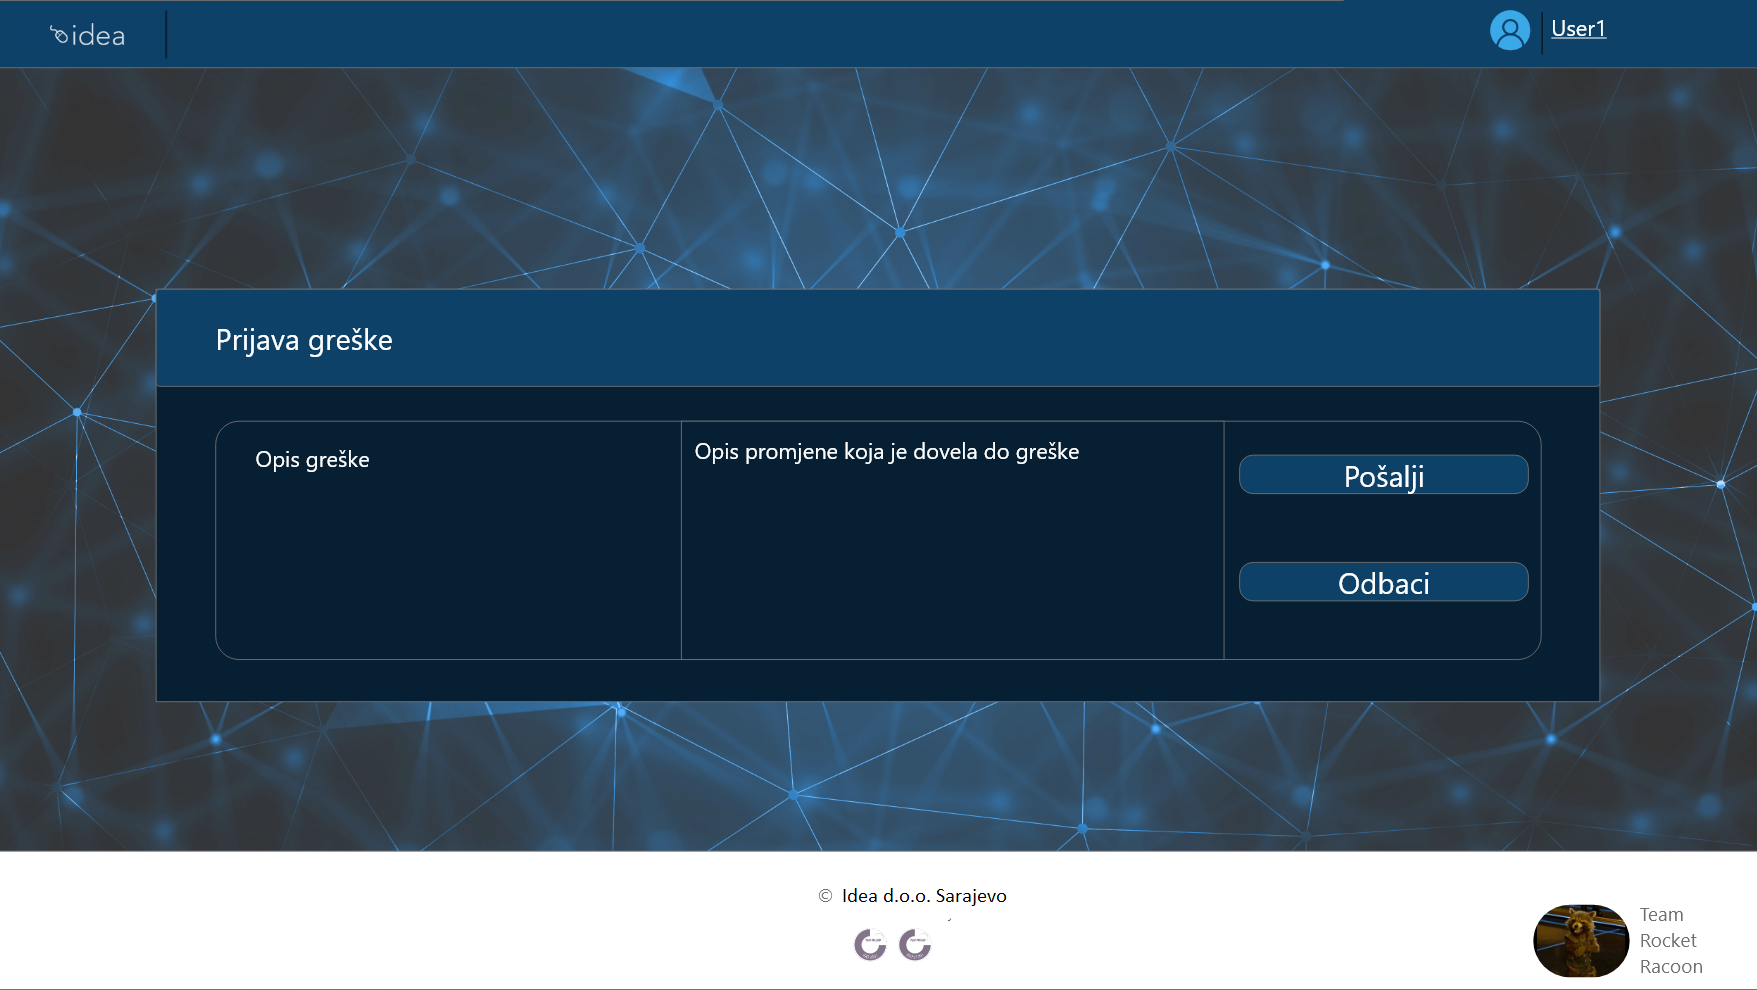
\includegraphics[scale=0.4]{../res/Prototype/Greske.PNG}
\caption{Izgled interfejsa za prijavu greške u sistemu}
\label{pt5}
\end{figure}

Na Slici \ref{pt6} prikazan je izgled ekrana za prijavu \textit{bug}-a od strane razvojnog tima. Nakon unosa neophodnih informacija, \textit{bug}-ovi se evidentiraju u sistemu kao događaji koje zatim pregleda tim za upravljanje promjenama te na koje adekvatno reaguje.

\begin{figure}[H]
\center
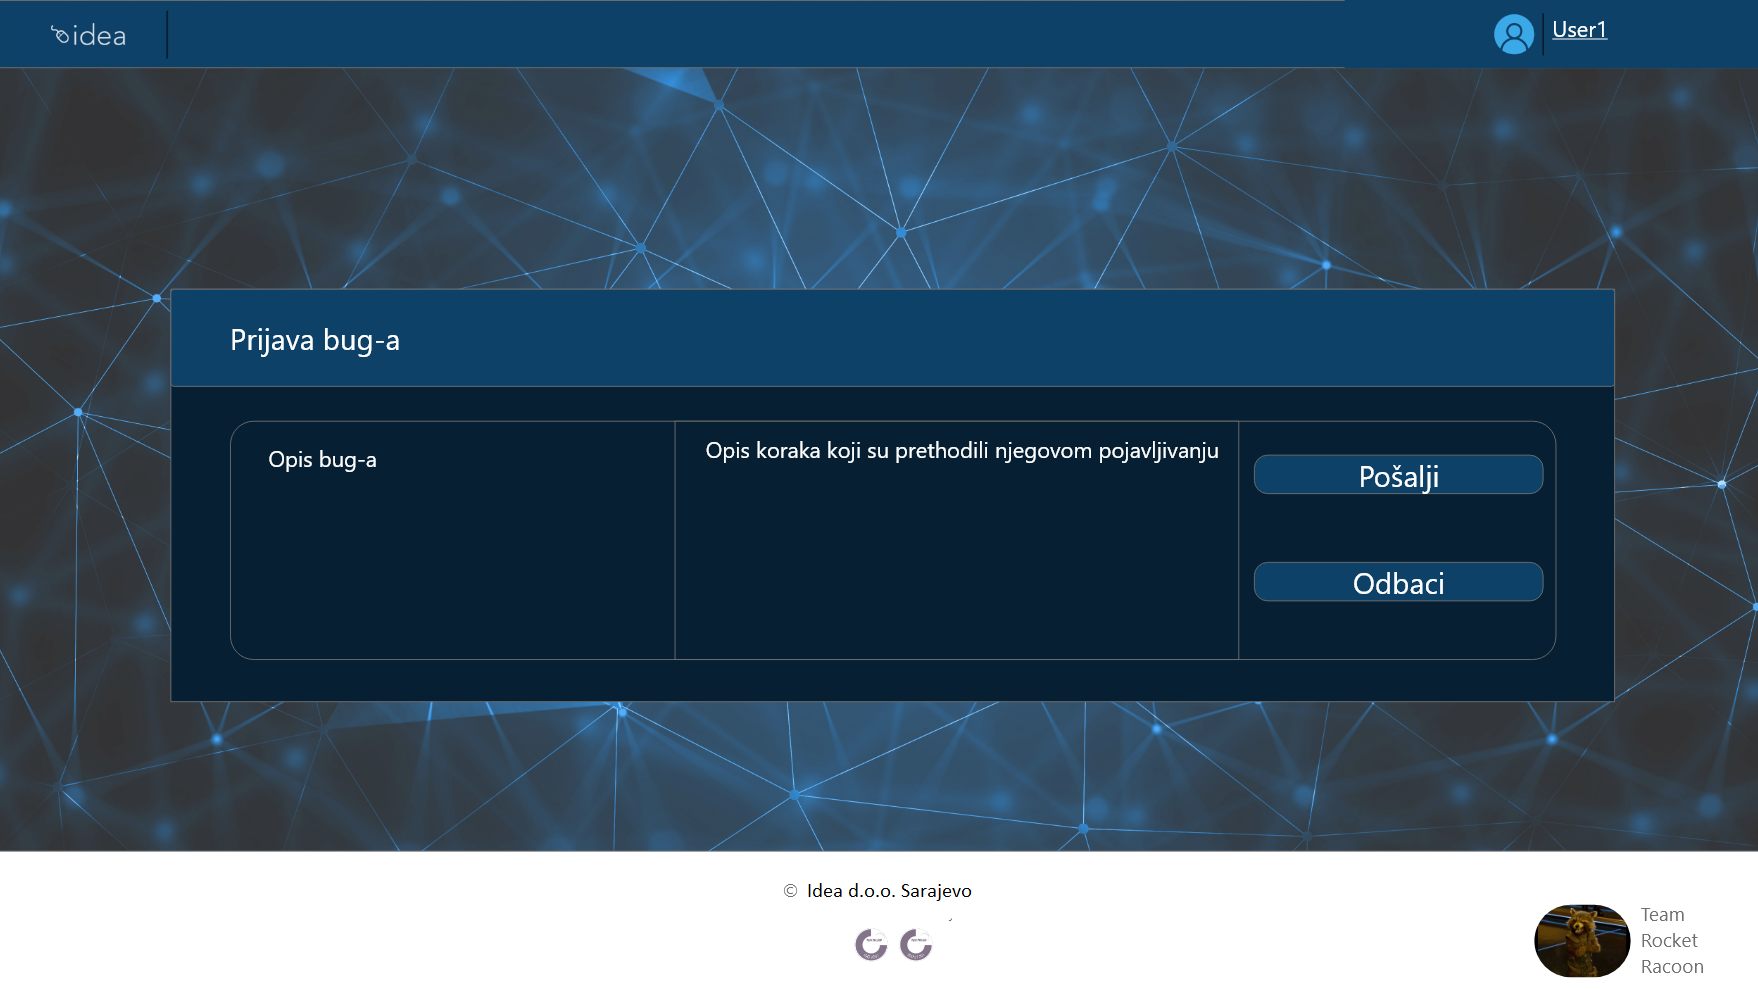
\includegraphics[scale=0.4]{../res/Prototype/Bugovi.PNG}
\caption{Izgled interfejsa za prijavu \textit{bug}-a u sistemu}
\label{pt6}
\end{figure}

\end{document}